\documentclass[12pt]{article}

% ======= Page & fonts =======
\usepackage[T1]{fontenc}
\usepackage[utf8]{inputenc}
\usepackage{lmodern}
\setlength{\oddsidemargin}{0.15in}
\setlength{\evensidemargin}{0.15in}
\setlength{\textwidth}{6.2in}
\setlength{\topmargin}{-0.5in}
\setlength{\textheight}{9in}
\linespread{1.06}

% ======= Math & symbols =======
\usepackage{amsmath,amssymb,amsfonts,bm,mathtools}
\usepackage{physics}
\usepackage{siunitx}
\sisetup{detect-all=true}
\usepackage{microtype}

% ======= Figures & TikZ =======
\usepackage{graphicx}
\usepackage{float}
\usepackage{caption}
\usepackage{subcaption}
\usepackage{tikz}
\usetikzlibrary{arrows.meta,positioning,calc,fit,decorations.markings,decorations.pathmorphing}

% ======= Hyperref & refs =======
\usepackage[colorlinks=true,linkcolor=blue,citecolor=blue,urlcolor=blue]{hyperref}
\usepackage{cite}

% ======= Macros: Canonical SST symbols (explicit; no undefined macros) =======
% constants (from Canon / user profile)
\newcommand{\vswirl}{\mathbf{v}_{\!\boldsymbol{\circlearrowleft}}}
\newcommand{\rc}{r_c}
\newcommand{\rhof}{\rho_{\!f}}
\newcommand{\rhocore}{\rho_{\text{core}}}
\newcommand{\rhoE}{\rho_{\!E}}
\newcommand{\rhoM}{\rho_{\!m}}
\newcommand{\bmvarrho}{\bm{\varrho}_{\!\boldsymbol{\circlearrowleft}}}
\newcommand{\Gsw}{\mathcal{G}_{\!\boldsymbol{\circlearrowleft}}}
\newcommand{\Ccanon}{C_e} % canonical swirl speed symbol in text

% handy display
\newcommand{\eqdef}{\coloneqq}

% ======= Title =======
\title{\Large\bfseries Rotating--Frame Unification in Swirl--String Theory:\\
Swirl--EMF Coupling, Flux Compression, and Quantized Impulses}

\author{Omar Iskandarani}
\date{\today}

\begin{document}
\maketitle

\begin{abstract}
We present a unified rotating--frame formulation in the Swirl--String Theory (SST) Canon in which time--varying vortex--line areal density $\bmvarrho$ acts as a \emph{source} of electromotive curl in Faraday's law,
\[
    \nabla\times\mathbf E=-\partial_t\mathbf B-\mathbf b_{\!\boldsymbol{\circlearrowleft}},
    \qquad
    \mathbf b_{\!\boldsymbol{\circlearrowleft}}=\Gsw\,\partial_t\bmvarrho.
\]
Topology fixes the time--integrated EMF impulse per net vortex event to be quantized:
\[
    \int dt\,\oint \mathbf E\!\cdot d\boldsymbol\ell=-\,\Gsw\,\Delta N,\quad \Delta N\in\mathbb Z,
\]
and canonical normalization yields $\Gsw=\Phi_\star\in\{h/e,\;h/2e\}$ \cite{Deaver1961,Doll1961}. With frozen line count, flux compression (shrinking area $A$) increases $\bmvarrho\propto 1/A$; when the mean spacing $a\sim \rc$ vortex nucleation bursts occur, producing EMF spikes consistent with the impulse law. We organize the manuscript by: (i) conceptual novelty and units, (ii) concise derivation and field diagram, (iii) predictions and falsifiers, with detailed derivations in Appendices~\ref{app:Faraday}–\ref{app:Impulse}, and a coil engineering appendix (Addendum~Q).
Non–original elements draw on \cite{Onsager1949,Feynman1955,LandauLifshitzEDCM,Deaver1961,Doll1961,Jacobson1995,Padmanabhan2010,Verlinde2011,Verlinde2017}.
\end{abstract}

\section{Introduction: Conceptual novelty}
    On SST leaves $\Sigma_t$ (absolute time $t$), particles are knotted vortex loops; circulation obeys the chronos--Kelvin invariant
    \begin{equation}
    \Gamma=\oint \vswirl\!\cdot d\boldsymbol\ell=N\kappa,\qquad N\in\mathbb Z,
    \label{eq:Kelvin}
    \end{equation}
    mirroring Onsager--Feynman quantization \cite{Onsager1949,Feynman1955}. The rotating--frame decomposition merges centrifugal and (swirl) gravity channels and motivates a long--range source $\mathbf b_{\!\boldsymbol{\circlearrowleft}}$ for $\nabla\times\mathbf E$. We show the unique linear, unit--consistent law
    \begin{equation}
    \boxed{\ \mathbf b_{\!\boldsymbol{\circlearrowleft}}=\Gsw\,\partial_t\bmvarrho\ }
    \label{eq:b-law}
    \end{equation}
    and fix $\Gsw$ by a flux–pumping pillbox argument to a flux quantum $\Phi_\star$ \cite{Deaver1961,Doll1961}. The prediction is falsifiable: EMF--time impulses are integer multiples of $\Phi_\star$ and tied to topological changes $\Delta N$.

\section{Framework, dimensions, and constitutive mirrors}
    Define the coarse--grained areal density (units $\mathrm{m^{-2}}$)
    \begin{equation}
    \bmvarrho(\mathbf x,t)\eqdef n_v(\mathbf x,t)\,\hat{\mathbf n},\qquad
    \Phi_{\!\boldsymbol{\circlearrowleft}}(A,t)=\int_A \bmvarrho\!\cdot d\mathbf A = N(A,t).
    \label{eq:rho-def}
    \end{equation}
    Local linear maps (laboratory tier) mirror standard electrodynamics \cite{LandauLifshitzEDCM}:
    \begin{equation}
    \mathbf D=\varepsilon\,\mathbf E,\ \ \mathbf B=\mu\,\mathbf H,
    \qquad
    \bmvarrho=\chi_H\,\mathbf H,\quad [\chi_H]=\mathrm{m^{-1}A^{-1}}.
    \label{eq:const-rel}
    \end{equation}
    Dimensional check: $[\partial_t\bmvarrho]=\mathrm{m^{-2}s^{-1}}$; since $[\nabla\times\mathbf E]=\mathrm{V\,m^{-2}}$, one needs $[\Gsw]=\mathrm{V\,s}=\mathrm{Wb}$ in \eqref{eq:b-law}. This sets the stage for a topological coupling normalized by a flux quantum.

\section{Rotating--frame unification and the swirl--EMF law}
    Starting from Faraday in differential form and appending the long–range source yields
    \begin{equation}
    \boxed{\ \nabla\times\mathbf E=-\partial_t\mathbf B-\mathbf b_{\!\boldsymbol{\circlearrowleft}},\quad
    \mathbf b_{\!\boldsymbol{\circlearrowleft}}=\Gsw\,\partial_t\bmvarrho\ }.
    \label{eq:Faraday-mod}
    \end{equation}
    Integrating over a surface $S$ with boundary $\partial S$ and time window $[t_i,t_f]$ gives the impulse law
    \begin{equation}
    \boxed{\ \int_{t_i}^{t_f}\!\!\oint_{\partial S}\mathbf E\!\cdot d\boldsymbol\ell\,dt
        =-\,\Gsw\,\Delta N(S)\ },\qquad \Delta N\in\mathbb Z.
    \label{eq:impulse}
    \end{equation}
    A single topological event ($\Delta N=\pm1$) generates a quantized EMF--time impulse of size $|\Gsw|$ regardless of geometry. Canonical normalization (Appendix~\ref{app:Faraday}) fixes $\Gsw=\Phi_\star\in\{h/e,h/2e\}$ \cite{Deaver1961,Doll1961}.

% ====== TikZ Diagram: Maxwell block with swirl link ======
    \begin{figure}[H]
    \centering
    \begin{tikzpicture}[
        node distance=1.6 and 2.2,
        every node/.style={draw, rounded corners, align=center, minimum height=2, font=\small},
        arrow/.style={-{Latex[length=2]}, thick},
        garrow/.style={-{Latex[length=2]}, thick, dashed}
    ]
    \node(Faraday)
    {$\nabla \times \mathbf{E} = -\,\partial_t \mathbf{B} \;-\; \mathbf{b}_{\!\boldsymbol{\circlearrowleft}}$\\
    \scriptsize $[\nabla\times\mathbf E]=\mathrm{V\,m^{-2}}$};
    \node[left=of Faraday]  (E)
    {$\mathbf{E}$\\ \scriptsize $[\mathbf E]=\mathrm{V\,m^{-1}}$};
    \node[right=of Faraday] (rho)
    {\scriptsize swirl density $\bmvarrho$\\ $[\bmvarrho]=\mathrm{m^{-2}}$};
    \node[below=of rho] (C)
    {$\bmvarrho = \chi_H\,\mathbf{H}$\\ \scriptsize $[\chi_H]=\mathrm{m^{-1}A^{-1}}$};
    \node[below=of E] (Ohm)
    {$\mathbf{j} = \sigma\,\mathbf{E}$\\ \scriptsize $[\sigma]=\mathrm{S\,m^{-1}}$};
    \node[below right=2.0 and -2.5 of Faraday] (B)
    {$\mathbf{B}=\mu\,\mathbf{H}$\\ \scriptsize $[\mu]=\mathrm{N\,A^{-2}}$};
    \node[below left=2.0 and -2.5 of Faraday] (D)
    {$\mathbf{D}=\varepsilon\,\mathbf{E}$\\ \scriptsize $[\varepsilon]=\mathrm{F\,m^{-1}}$};
    \node[below=of Ohm] (J)
    {$\mathbf{j}$\\ \scriptsize $[\mathbf j]=\mathrm{A\,m^{-2}}$};
    \node[right=of J] (Ampere)
    {$\nabla \times \mathbf{H} = \mathbf{j} + \partial_t \mathbf{D}$\\
    \scriptsize $[\nabla\times\mathbf H]=\mathrm{A\,m^{-2}}$};
    \node[below=of C] (H)
    {$\mathbf{H}$\\ \scriptsize $[\mathbf H]=\mathrm{A\,m^{-1}}$};
    \node[above left=1.2 and 0.6 of rho] (b)
    {$\mathbf{b}_{\!\boldsymbol{\circlearrowleft}}=\Gsw\,\partial_t\bmvarrho$\\ \scriptsize $[\mathbf b]=\mathrm{V\,m^{-2}}$};
    \draw[arrow] (E) -- (D);
    \draw[arrow] (C) -- (rho);
    \draw[arrow] (rho) -- (Faraday);
    \draw[arrow] (J) -- (Ampere);
    \draw[arrow] (H) -- (Ampere);
    \draw[arrow] (E) -- (Faraday);
    \draw[arrow] (Faraday) -- (B);
    \draw[arrow] (Ampere) -- (D);
    \draw[arrow] (B) -- (H);
    \draw[arrow] (H) -- (C);
    \draw[arrow] (E) -- (Ohm);
    \draw[arrow] (Ohm) -- (J);
    \draw[garrow] (rho.south west) -- node[above,sloped,inner sep=1pt]
        {\scriptsize long–range mediation} (b.north);
    \draw[arrow] (b) -- (Faraday);
    \end{tikzpicture}
    \caption{Constitutive mirrors and the added long–range swirl source in Faraday’s law.}
    \label{fig:diagram}
    \end{figure}

\section{Flux compression and nucleation (kept; empirical VAM table dropped)}
    With total line count $N$ frozen,
    \begin{equation}
    \bmvarrho(A)=\frac{N}{A}\,\hat{\mathbf n},\qquad
    n_v=\frac{N}{A},\qquad
    a\sim n_v^{-1/2}=\sqrt{\frac{A}{N}}.
    \label{eq:flux-compress}
    \end{equation}
    Nucleation occurs when $a\lesssim \alpha\,\rc$:
    \begin{equation}
    n_v\gtrsim (\alpha\,\rc)^{-2}.
    \label{eq:nucl}
    \end{equation}
    In a rotating bucket, $n_v\simeq 2\Omega/\kappa$ \cite{Feynman1955}, providing a rotation–dependent threshold. During nucleation bursts, $\partial_t\bmvarrho\neq 0$, so $\mathbf b_{\!\boldsymbol{\circlearrowleft}}\neq 0$ and EMF impulses follow \eqref{eq:impulse}.

% ====== TikZ: plate shrink schematic ======
    \begin{figure}[H]
    \centering
    \begin{tikzpicture}[scale=1.0, >=Latex]
    \draw[very thick] (-5,1.2) rectangle (-1,-1.2);
    \node at (-3,1.5) {$A_0$};
    \foreach \x in {-4.5,-3.4,-2.2}{
        \draw[very thick] (\x,-1.0) -- (\x,1.0);
        \draw[fill=black] (\x,0) circle (0.05);
    }
    \node[align=center] at (-3,-1.6)
        {$\Phi_{\!\boldsymbol{\circlearrowleft}}=N\kappa$};

    \draw[very thick] (1.0,0.8) rectangle (4.0,-0.8);
    \node at (2.5,1.1) {$A$};
    \foreach \x in {1.3,1.8,2.3,2.8,3.3}{
        \draw[very thick] (\x,-0.7) -- (\x,0.7);
        \draw[fill=black] (\x,0) circle (0.05);
    }
    \draw[->,thick] (-0.3,0) -- (0.3,0) node[midway,above] {shrink};
    \node[align=left] at (5.0,0.6)
        {$\bmvarrho(A)=\dfrac{N}{A}\,\hat{\mathbf n}$};
    \node[align=left] at (5.0,0.0)
        {$n_v=\dfrac{N}{A},\ a\sim n_v^{-1/2}$};
    \node[align=left] at (5.0,-0.6)
        {$a\lesssim \alpha \rc\ \Rightarrow\ \text{nucleation}$};
    \end{tikzpicture}
    \caption{Fixed swirl flux, shrinking area $\Rightarrow$ increased $\bmvarrho$ and nucleation at $a\sim \rc$.}
    \label{fig:plates}
    \end{figure}

\section{Predictive power: experimental outlook}
    \paragraph{Quantized impulse (primary observable).}
        \begin{equation}
        \int dt\,\mathrm{EMF}(t)=\Phi_\star\,\Delta N,\qquad
        \Phi_\star\in\{h/e,\ h/2e\}.
        \label{eq:obs}
        \end{equation}
    \paragraph{Platforms.} (i) Type–II superconducting films with controlled single–vortex entry/exit and SQUID pickup \cite{Deaver1961,Doll1961}; (ii) superfluid vortex nucleation/annihilation \cite{Feynman1955}; (iii) magnetic topological textures (skyrmion nucleation/erasure) as analogs.
    \paragraph{Falsifiers.} (a) Histogram of $\Delta\Phi=\int V(t)dt$ exhibits integer peaks at $\Phi_\star$ (no fractional plateaus); (b) sign flips with chirality; (c) topology dependent, geometry independent; (d) unlinking eliminates the signal.

\section{Conclusion \& discussion}
Equations \eqref{eq:Faraday-mod}–\eqref{eq:impulse} provide a minimal, unit–consistent bridge from rotating–frame vortex dynamics to EM induction. The integrated impulse $\Phi_\star\,\Delta N$ is a sharp, falsifiable signature already compatible with existing single–vortex control. Determining whether $\Phi_\star=h/2e$ or $h/e$ is a material/topology discriminator. Full derivations are in Appendices.

% ====================== APPENDICES ======================
\appendix

\section*{Appendix A: Modified Faraday law from swirl flux pumping}
\label{app:Faraday}
Start with integral Faraday:
\begin{equation}
\oint_{\partial S}\mathbf E\!\cdot d\boldsymbol\ell
=-\frac{d}{dt}\int_S\mathbf B\!\cdot d\mathbf A.
\label{eq:Faraday-int}
\end{equation}
Define $N(t)=\int_S \bmvarrho\!\cdot d\mathbf A$ and a swirl–flux term $\Phi_{\!\boldsymbol{\circlearrowleft}}=\Gsw\,N$. Then
\begin{align}
\oint_{\partial S}\mathbf E\!\cdot d\boldsymbol\ell
&=-\frac{d\Phi_B}{dt}-\frac{d\Phi_{\!\boldsymbol{\circlearrowleft}}}{dt}
\nonumber\\
&=-\int_S \partial_t\mathbf B\!\cdot d\mathbf A\ -\ \Gsw\int_S \partial_t\bmvarrho\!\cdot d\mathbf A.
\end{align}
By Stokes, $\int_S [\nabla\times\mathbf E+\partial_t\mathbf B+\Gsw\,\partial_t\bmvarrho]\!\cdot d\mathbf A=0$ for arbitrary $S$, giving \eqref{eq:Faraday-mod}. Choosing $\Gsw=\Phi_\star$ aligns one net event with one flux quantum \cite{Deaver1961,Doll1961}.

\section*{Appendix B: Flux compression $\Rightarrow$ nucleation threshold}
\label{app:Threshold}
With $N$ frozen, \eqref{eq:flux-compress} gives $a=\sqrt{A/N}$; the onset condition $a\lesssim\alpha\rc$ implies
\begin{equation}
\frac{N}{A}\gtrsim\frac{1}{\alpha^2\rc^2}.
\end{equation}
In a rotating frame, the Feynman relation $n_v\simeq 2\Omega/\kappa$ \cite{Feynman1955} yields a rotation–dependent threshold $A_\star(\Omega)\simeq N\,\kappa/(2\Omega)$.

\section*{Appendix C: Impulse quantization and choice of $\Phi_\star$}
\label{app:Impulse}
Integrate \eqref{eq:Faraday-mod} over $S$ and $[t_i,t_f]$:
\begin{equation}
\int_{t_i}^{t_f}\!\!\oint_{\partial S}\mathbf E\!\cdot d\boldsymbol\ell\,dt
=-\int_{t_i}^{t_f}\!\!\int_S \partial_t\mathbf B\!\cdot d\mathbf A\,dt\ -\ \Gsw\int_{t_i}^{t_f}\!\!\int_S \partial_t\bmvarrho\!\cdot d\mathbf A\,dt.
\end{equation}
Holding $\Phi_B$ fixed gives $\int dt\,\oint \mathbf E\!\cdot d\boldsymbol\ell=-\Gsw\,\Delta N$. Thus impulses are quantized in units of $|\Gsw|$, and canonical choices are $\Phi_\star=h/2e$ (superconducting flux quantum) or $h/e$ \cite{Deaver1961,Doll1961}.

% ====================== ADDENDUM Q ======================
\section*{Appendix D (Addendum Q): Double--Saw--Shaped Coil Stack Realization}
\label{sec:addendumQ}
\subsection*{Q.1 Definition (Double--Saw--Shaped Coil)}
    On a stator with $S=40$ slots and $p=4$ poles, consider a short--pitched 3--phase winding with pitch $y=2$ (step rule $+11/ -9$). The chording angle
    \[
        \gamma = y\,\alpha_e = 36^\circ,\qquad
        \alpha_e = \frac{180^\circ p}{S} = 18^\circ,
    \]
    implies $k_p^{(5)}=\cos(\tfrac{5\gamma}{2})=0$. Implement two interleaved 3--phase saw--shaped coils (``Double--Saw--Shaped''), with electrical displacement $\Delta_e=30^\circ$,
    \[
        \mathcal A_\nu \propto 2\cos\!\Big(\frac{\nu\Delta_e}{2}\Big)\,k_w^{(\nu)}\!,
    \]
    hence $\mathcal A_1 \approx 1.93\,k_w^{(1)}$, $\mathcal A_5=0$, $\mathcal A_6=0$, $\mathcal A_7\simeq -0.05$.

\subsection*{Q.2 Stacking (Two Double--Saw--Shapeds)}
    Place two identical Double--Saw--Shaped coils axially stacked (gap $h$), on--axis contributions $B_T(z)$, $B_B(z)$. Canonical modes:
    \begin{align*}
    \text{Mode A (additive):}&\ \ B_{\textrm tot}\simeq B_T+B_B \Rightarrow \text{max fundamental},\\
    \text{Mode B (gradient):}&\ \ \Delta p = \eta\,\tfrac{B_B^2-B_T^2}{2\mu_0} \Rightarrow \text{effective gravity blocking},\\
    \text{Mode C (counter--rot.):}&\ \ B_{\textrm rot}\to 0,\ \nabla B^2\neq 0 \Rightarrow \text{standing pressure pattern},\\
    \text{Mode D (beat):}&\ \ \varphi\neq 0 \Rightarrow \text{axially traveling envelope}.
    \end{align*}

\subsection*{Q.3 Canonical Equation (Swirl Pressure)}
    Within the SST Canon,
    \[
        p_{\textrm sw}(z) = \eta\,\frac{\langle B^2(z)\rangle}{2\mu_0},
    \]
    so a stacked asymmetry yields
    \[
        F_z = \int_A \Delta p(z)\,dA
        =\eta\;\frac{B_B^2-B_T^2}{2\mu_0}\,A.
    \]

\subsection*{Q.4 Experimental Pathway}
    \begin{enumerate}\itemsep2pt
    \item Verify harmonic hygiene: $5^{\textrm th}=0$, $6^{\textrm th}=0$, $7^{\textrm th}\ll1$.
    \item Map $B(z)$ with Hall sensors for both stacks.
    \item Tune $B_B/B_T$ to measure $\Delta p$ on a plate of area $A$.
    \item Switch to Mode~C (counter--rotate top stack) to confirm $\nabla B^2$ persists with vanishing torque.
    \end{enumerate}

\subsection*{Q.5 Canonical Status}
    This configuration satisfies Canon hygiene and realizes swirl pressure modulation for gravity--blocking tests.

% ====================== Bibliography ======================
    \bibliographystyle{unsrt}
    \begin{thebibliography}{99}

    \bibitem{Onsager1949}
    L.~Onsager,
    Statistical hydrodynamics,
    \emph{Il Nuovo Cimento (Suppl.)} \textbf{6}, 279 (1949).

    \bibitem{Feynman1955}
    R.~P. Feynman,
    Application of Quantum Mechanics to Liquid Helium,
    in \emph{Progress in Low Temperature Physics}, Vol.~I, 17--53 (1955).

    \bibitem{LandauLifshitzEDCM}
    L.~D. Landau and E.~M. Lifshitz,
    \emph{Electrodynamics of Continuous Media}, 2nd ed.,
    Pergamon (1984).

    \bibitem{Deaver1961}
    B.~S. Deaver Jr., W.~M. Fairbank,
    Experimental Evidence for Quantized Flux in Superconducting Cylinders,
    \emph{Phys. Rev. Lett.} \textbf{7}, 43 (1961).

    \bibitem{Doll1961}
    R.~Doll, M.~N{\"a}bauer,
    Experimental Proof of Magnetic Flux Quantization in a Superconducting Ring,
    \emph{Phys. Rev. Lett.} \textbf{7}, 51 (1961).

    \bibitem{Jacobson1995}
    T.~Jacobson,
    Thermodynamics of Spacetime: The Einstein Equation of State,
    \emph{Phys. Rev. Lett.} \textbf{75}, 1260 (1995).

    \bibitem{Padmanabhan2010}
    T.~Padmanabhan,
    Thermodynamical Aspects of Gravity: New Insights,
    \emph{Rep. Prog. Phys.} \textbf{73}, 046901 (2010).

    \bibitem{Verlinde2011}
    E.~P. Verlinde,
    On the Origin of Gravity and the Laws of Newton,
    \emph{JHEP} \textbf{2011}(4):29 (2011).

    \bibitem{Verlinde2017}
    E.~P. Verlinde,
    Emergent Gravity and the Dark Universe,
    \emph{SciPost Phys.} \textbf{2}, 016 (2017).

    \end{thebibliography}

\end{document}
